\chapter{Data}

There are 3 types of data we can use to test the accuracy and reliability of the script. Iridium flares can be predicted, allowing one to prepare to collect their data. NASA data can provide a steady source of fireball events to access along with their data to compare to. Finally, fireball events detected by D6 will be tested.

\section{Iridium Flares}

The first step in testing out the script is to run it in conjunction with video collected directly from D6. A simple way to do this is to run it against a video clip of an Iridium flare that D6 captured. There are two benefits of testing against an Iridium flare. First, Iridium flares are predicted online and their maximum magnitudes are recorded. We can find the maximum value from our light curve and compare it to the known maximum magnitude. Second, the light curves from Iridium flares are very smooth, and the flare moves a minimal amount, reducing risk of errors due to tracking. This makes it easy to notice any discrepancies in individual frames. We have collected two Iridium flare events using D6. 

In late November of 2017, D6 was able to capture an Iridium flare going over Collins Hall at Willamette University in Salem, Oregon. The first frame of this event is shown as Figure~\ref{fig:Iridium}.
\begin{figure}[ht!]
	\centering
	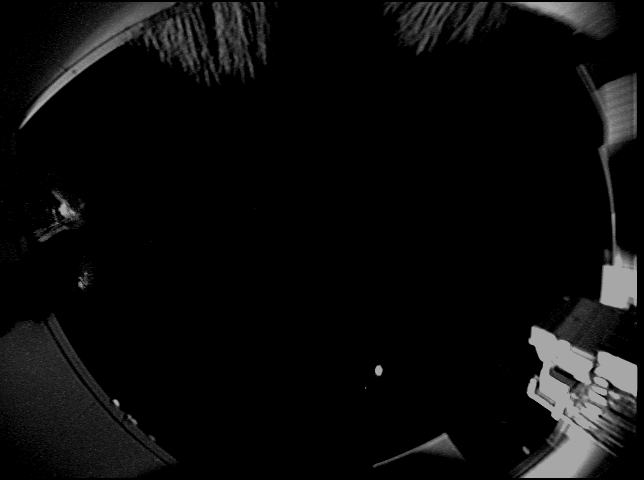
\includegraphics[width=0.6\linewidth]{iridium.png}
	\caption{The first Iridium flare captured by D6 at Willamette University.}
	\label{fig:Iridium}
\end{figure}
 Its light curve was then created, shown in Figure~\ref{fig:IridiumCurves}.
\begin{figure}
\centering
\begin{subfigure}{.5\textwidth}
	\centering
	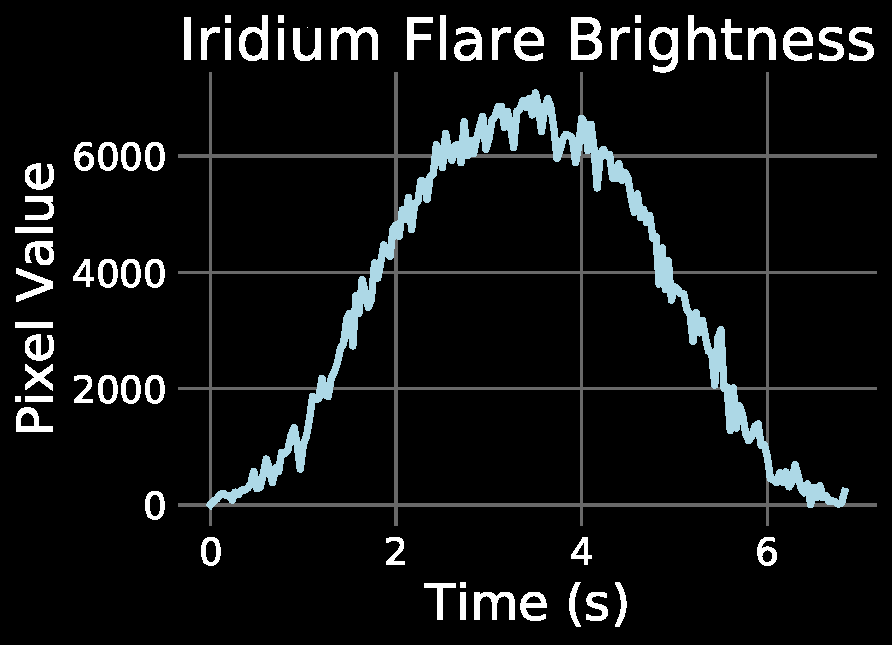
\includegraphics[width=\linewidth]{/home/luke/Data/IridiumFlare/IridiumMag.pdf}
	\label{fig:Iridiummag}
\end{subfigure}%
\begin{subfigure}{.5\textwidth}
	\centering
	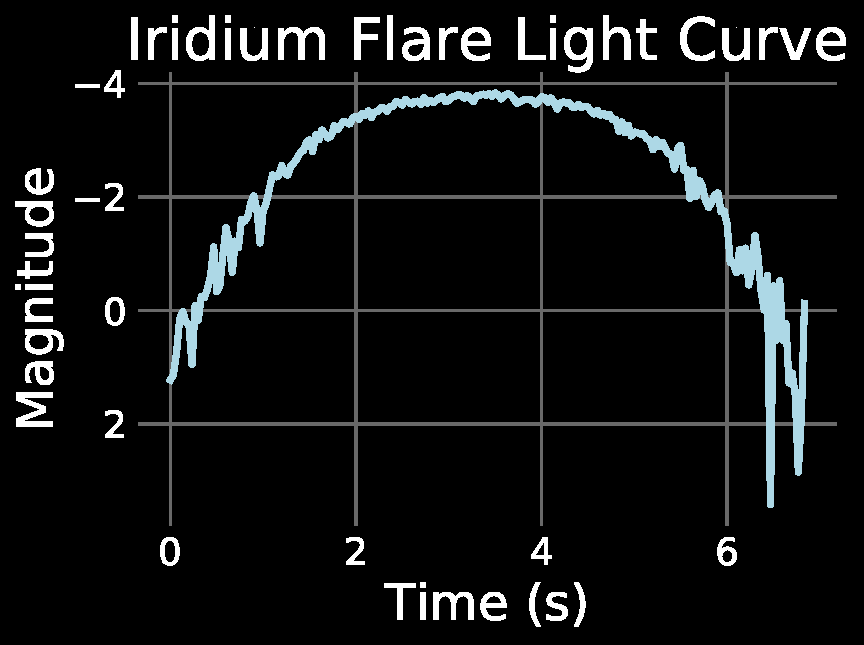
\includegraphics[width=\linewidth]{/home/luke/Data/IridiumFlare/IridiumCurve.pdf}
	\label{fig:Iridiumcurve}
	\end{subfigure}
\caption{While light curves are usually displayed in terms of magnitude, it's important to remember the source of those magnitude values: pixel values.}
\label{fig:IridiumCurves}
\end{figure}

The first thing to check is if it qualitatively agrees with visual inspect of the event's video. The Iridium flare's brightness seems to dramatically increase before dimming away. The light curves shown in Figure~\ref{fig:IridiumCurves} agree with that assessment. So in a qualitative sense, the photometry program is capable of tracking the event and measuring its light. 

Some issues did emerge from this event, however. Ideally, we would like to be able to compare the maximum magnitude from the light curve our program created to the recorded maximum magnitude of the event. Unfortunately, the Iridium flare was so bright that it oversaturated our camera. This can be seen in Figure~\ref{fig:ObjectPlot055}.
\begin{figure}[ht!]
	\centering
	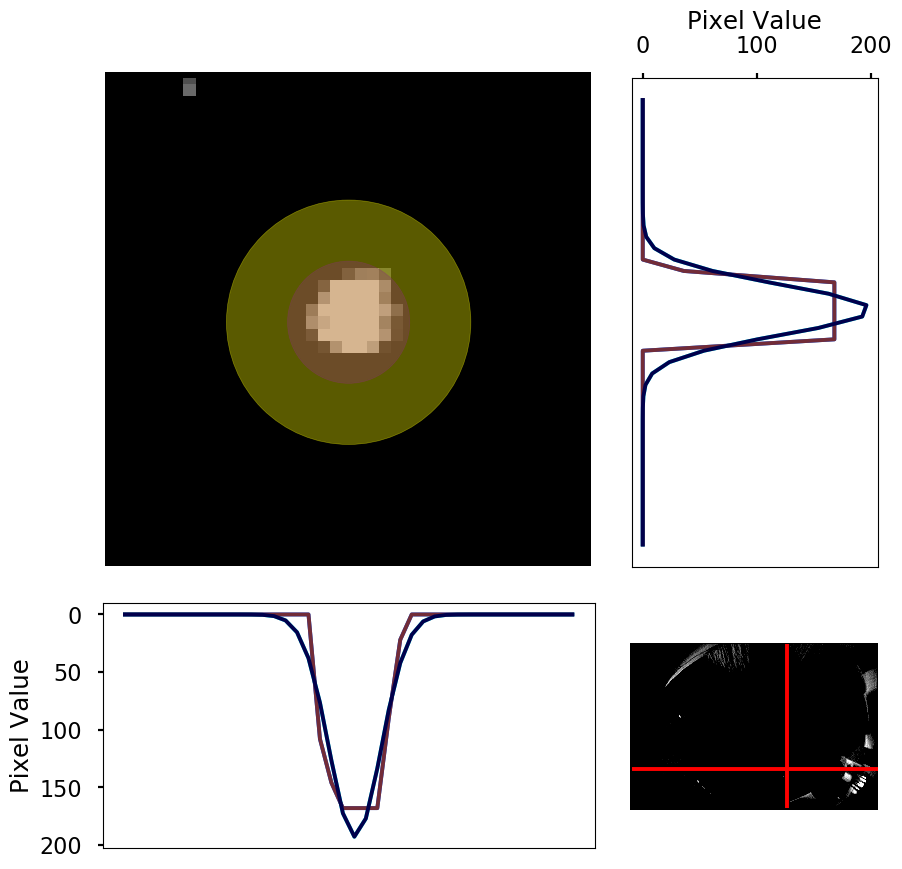
\includegraphics[width=0.4\linewidth]{ObjectPlotInverse.png}
	\caption{The X and Y data slices are plotted alongside the object. The peak of the event flattens out, when one would expect it to curve at the top, similar to the Gaussian fittings fitted upon the data.}
	\label{fig:ObjectPlot055}
\end{figure}
Figure~\ref{fig:ObjectPlot055} allows us to see that the center of event is too bright for our camera's sensors. As a result, we are unable to find the current maximum magnitude of that Iridium flare event. This saturation also explains why the peaks in Figure~\ref{fig:Iridiumcurve} and Figure~\ref{fig:Iridiummag} last for a substantial portion of the event; the true peak brightness isn't visible on those graphs. As a result, this light curve would be underestimating the true peak brightness of the event.

Another issue that is apparent in the Iridium flare data is noise appearing in sections of the data. Specifically, the noise at the end of the event appears most jarring in Figure~\ref{fig:IridiumCurves} when the logarithm is applied. When the event nears its end, the signal to noise ratio greatly decreases. This noise is a result of the background light that has already been mentioned. Since the event is at its end, it is becoming incredibly dim, and in its last moments its signal is basically equal with the background light around it. Since the background light value we are using is the average of the area around the event, there arises occasions where the pixels of the event are smaller than the background light at this stage. This creates a magnitude that is the resultant of a log of an incredibly small, or even negative number. Since taking the logarithm of a negative error is mathematically impossible, those values are set to 0. So, at the end of an event before the program no longer detects any trace of the event, the last data points are very small, and that smallness is magnified by the logarithm.

Iridium flares are somewhat useful pseudo-meteors, but ultimately the program needs to show that it can successfully track actual meteors. When running the program on an Iridium flare event, the tracking algorithm is not challenged greatly; the flare's light was at a relatively constant position on the camera's frames. Meteor events that do move far across the screen pose a new challenge for the program that needs testing.

\section{Comparison to NASA Data}

The methods section provided an example of a light curve acquired from our program using a NASA video clip. By running the script against videos of events recorded by NASA, we can confirm that the script is working by comparing it to NASA's light curves provided with the videos. The collected data and results of this test are discussed below.

The first event that we acquired from NASA's database was one that occurred on March 21, 2018, by one of their cameras stationed in Central Florida. The video was downloaded alongside their infographic of data involving the event. This infographic, displayed as Figure~\ref{fig:infographic} contains the light curve of the event in the top right corner. 
\begin{figure}[ht!]
	\centering
	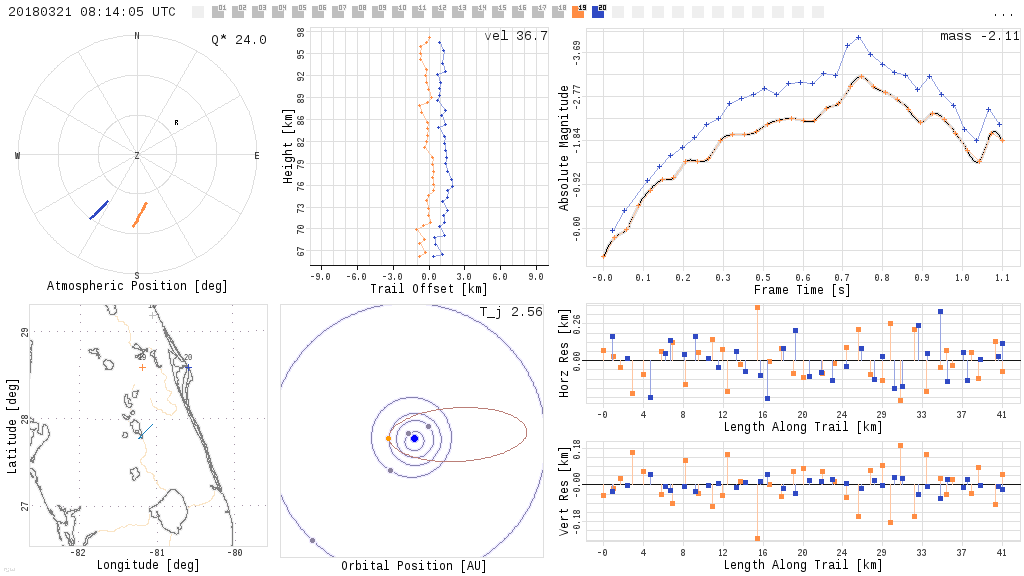
\includegraphics[width=.75\linewidth]{infographicinverse.png}
	\caption{The light curve NASA attained off the same video is shown in orange in the top right of the graphic.}
	\label{fig:infographic}
\end{figure}
In order to convert that picture of the light curve to a dataset we can work with, the light curve was run through a plot digitizer to extract the numerical data and convert it to a CSV file.

While the light curve is crucial to compare our results to, the infographic also contains crucial information for star calibration such as the video's location, the event's direction, and the time of the event. This allows us to make use of planetarium software to view how the stars were positioned at that time and orientation, so we can identify a valid reference star. For our purposes, we used Stellarium. Stellarium is a free, open-source\footnote{Open-source projects are one the best catalysts of intelligent thought in a society. If possible, they should be used at all costs} planetarium available on all three major operating systems\footnote{Available on most, but perhaps not all, Linux distributions}.

With Stellarium, we were able to obtain a view of the position of celestial objects at that time, as seen in Figure~\ref{fig:Starposition}.
\begin{figure}
\centering
\begin{subfigure}{.4\textwidth}
	\centering
	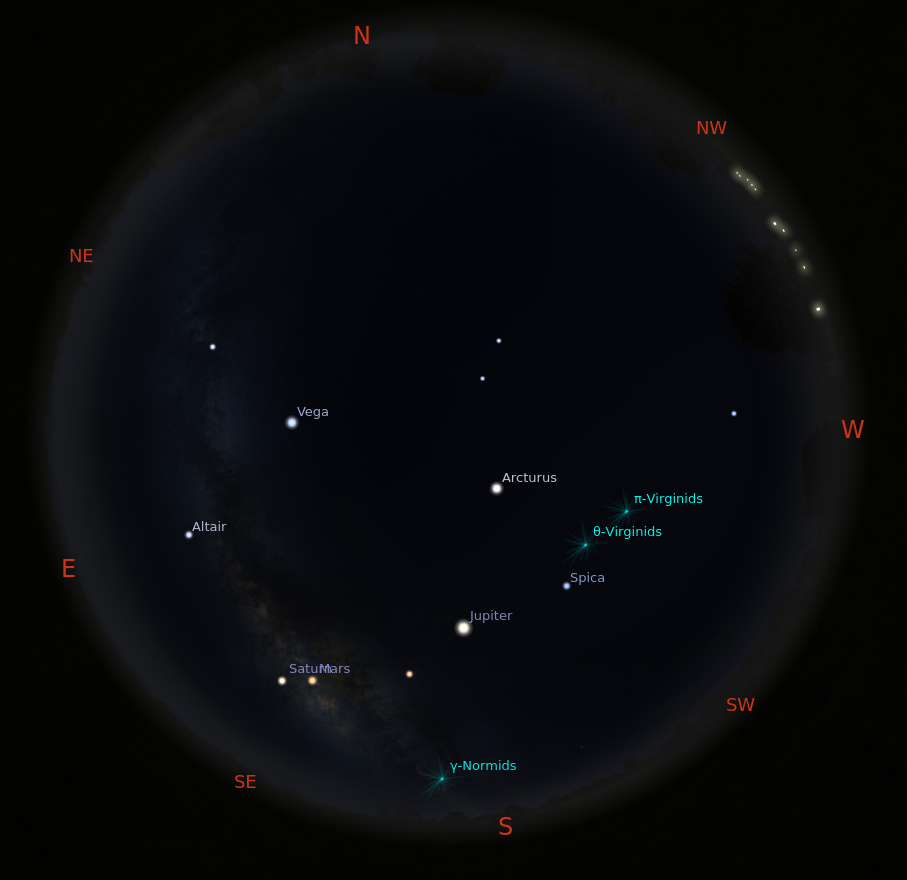
\includegraphics[height=.85\linewidth]{stellarium}
\end{subfigure}%
\begin{subfigure}{.4\textwidth}
	\centering
	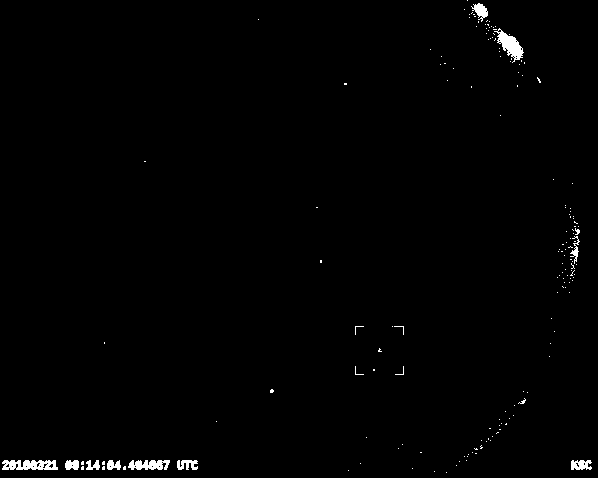
\includegraphics[height=.85\linewidth]{ThresholdFrame.png}
\end{subfigure}
\caption{The thresholded image with labels added next to identified objects, next to the Stellarium image it was compared to.}
\label{fig:Starposition}
\end{figure}
The Stellarium image in Figure~\ref{fig:Starposition} was then compared to the thresholded video frames of the event in order to try to identify one of the brighter objects. Assuming the Stellarium was positioned correctly, celestial objects should appear to be in the same place in both images. A few pieces of data can be extracted from the two images. The only piece of data that we need is the magnitude of a single object, which can be obtained by clicking on that object in Stellarium. For this calibration, Jupiter was used with its magnitude of -2.35 at the time. Another piece of data that can be extracted is that the event in question was most likely from the $\theta$-Virginids or $\pi$-Virginids, as the event is in the same area as those two meteor showers were on that day. This is another piece of strong evidence that the sky is oriented correctly in the images.

Now that we had a celestial object with a magnitude to calibrate to, the program was ran on the event. When it finished, the end result is the magnitude of each frame plotted over the time of the event, showing the light curve of the event. The light curve of this event from the program is shown in Figure~\ref{fig:nasa}. 
\begin{figure}[ht!]
	\centering
	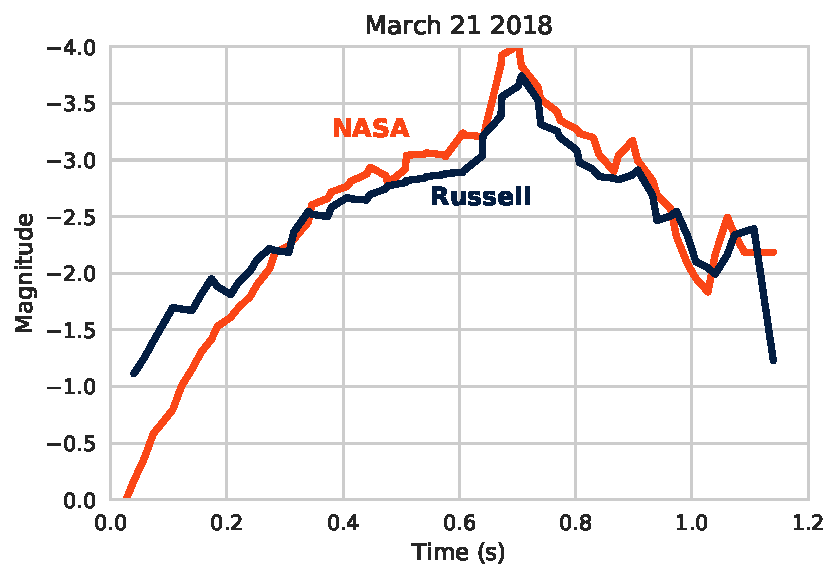
\includegraphics[width=0.6\linewidth]{LightCurveComparison.pdf}
	\caption{The event in question is the light curve on the top.}
	\label{fig:nasa}
\end{figure}
The general trend shows that program's methodology in calculating the magnitude is sound. We would expect the brightness to gradually grow before diminishing again, and the graph agrees with that. This event in question was detected off from one of NASA's cameras. As a result, we can compare our light curve to NASA's to double check. NASA's light curve can also be seen in Figure~\ref{fig:nasa}. They are pretty similar.


One aspect of the data that does not seem to fit well is the beginning of the event. This can be seen quantitatively by plotting the residuals of the two data sets and looking for outliers, which is done in Figure~\ref{fig:residuals1}.
\begin{figure}[ht!]
	\centering
	\includegraphics[width=0.6\linewidth]{/home/luke/Data/NASA/2018-03-21-0814/201803210814Residuals.pdf}}
	\caption{Caption}
	\label{fig:residuals1}
\end{figure}
The difference in the two plots can also be displayed with the use of a violin plot, shown in Figure~\ref{fig:violinplot}. This allows us to see whether it is overestimating or underestimating the magnitude by looking at the top and bottom of the plot. By accounting for the offset, those outliers are not masked underneath a consistent offset some data may have.
\begin{figure}[ht!]
	\centering
	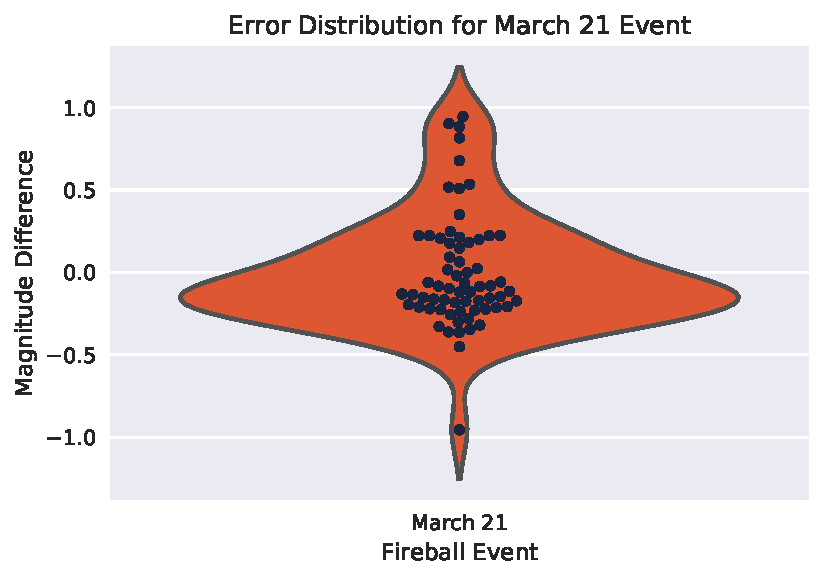
\includegraphics[width=0.6\linewidth]{ViolinPlot1.pdf}
	\caption{Testviolinplot}
	\label{fig:violinplot}
\end{figure}

Light curve comparisons and the responding violin plots were then made for other events pulled from NASA's all-sky camera network. The light curves are shown in Figure~\ref{fig:lightcurves}.
\begin{figure}[ht!]
\centering
\begin{subfigure}{.45\textwidth}
  \centering
  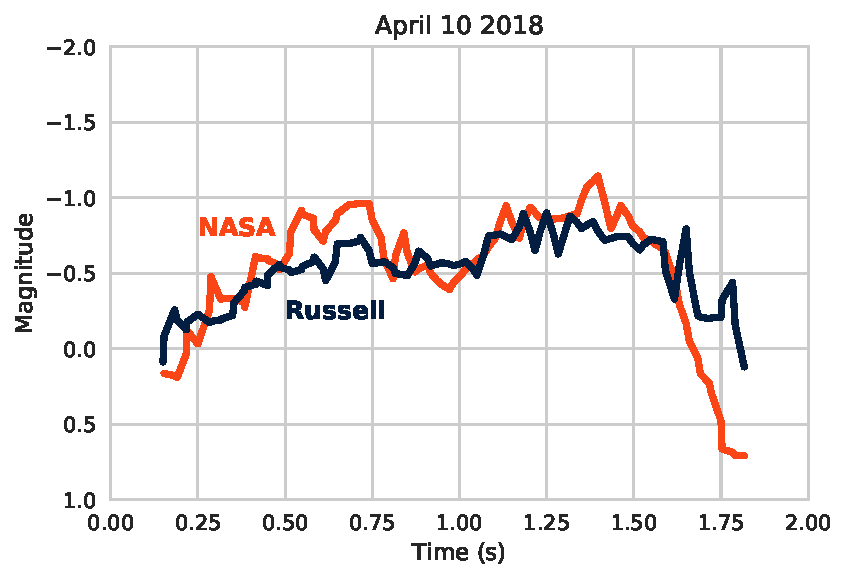
\includegraphics[width=\linewidth]{LightCurveComparison2.pdf}
  \label{fig:nothresholdd6}
\end{subfigure}%
\begin{subfigure}{.45\textwidth}
  \centering
  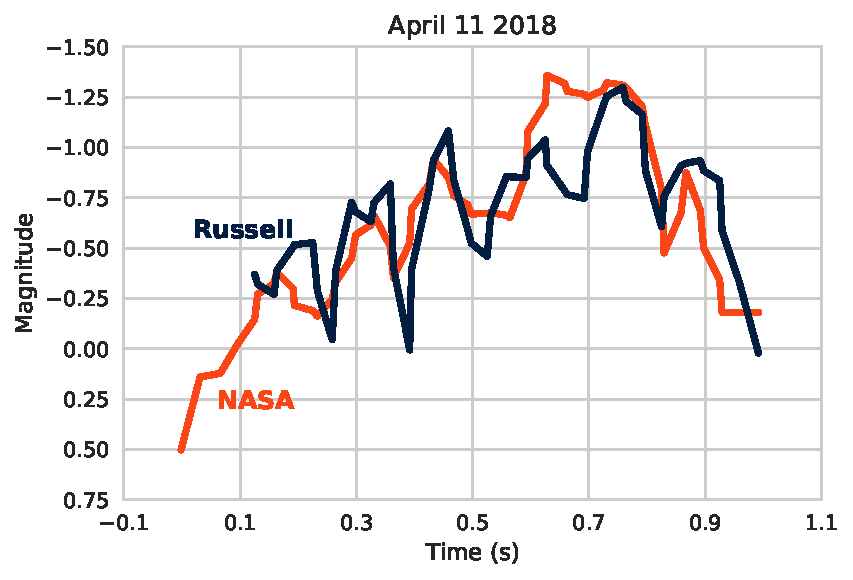
\includegraphics[width=\linewidth]{LightCurveComparison3.pdf}
  \label{fig:thresholdd6}
\end{subfigure}
\begin{subfigure}{.45\textwidth}
  \centering
  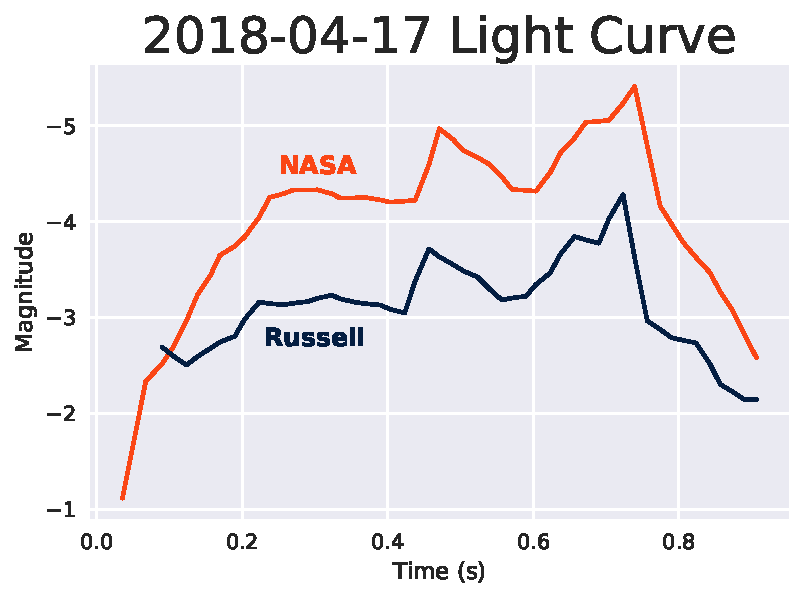
\includegraphics[width=\linewidth]{LightCurveComparison4.pdf}
  \label{fig:thresholdd6}
\end{subfigure}
\begin{subfigure}{.45\textwidth}
  \centering
  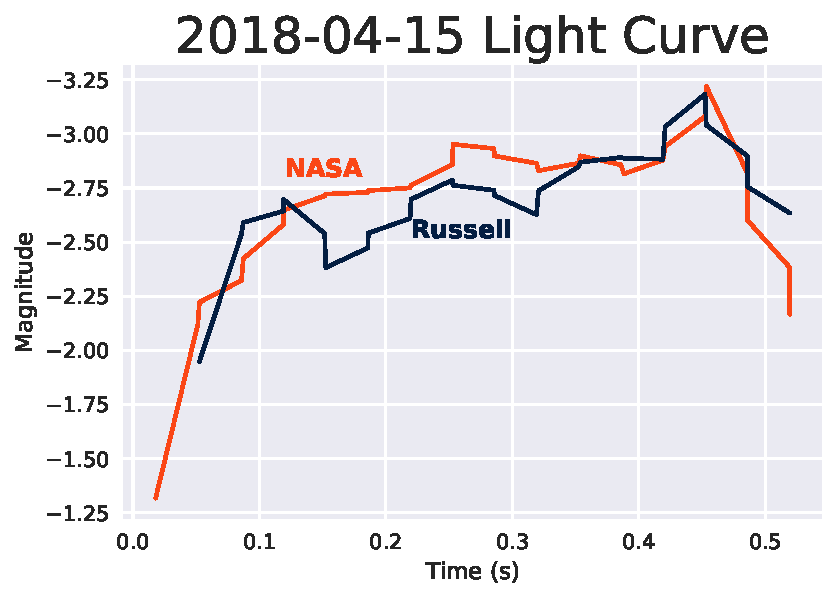
\includegraphics[width=\linewidth]{LightCurveComparison5.pdf}
  \label{fig:thresholdd6}
\end{subfigure}
\caption{Light curves collected over multiple events.}
\label{fig:lightcurves}
\end{figure}
Again, it should be stated that the Y-axes of these graphs are shifted magnitude, as the NASA light curves were shifted up for comparison purposes once again. The choppiness of some of the curves, specifically the one for the April 11 event, makes it somewhat difficult to see how much the two light curves agree with other.

As a result, violin plots were made for the datasets again. This is seen in Figure~\ref{fig:twoviolin}. The results were generally in agreement with each other, with a few points being outliers once again, specifically for the events on March 21 and April 10. In order to get a general idea on the accuracy in the aggregate, Figure~\ref{fig:twoviolin} also shows the combined violin plot. Again, there a few outliers, but in general the data are in agreement, with the majority of the points being within 0.5 magnitude in either direction of the mean.
\begin{figure}[ht!]
\centering
\begin{subfigure}{.5\textwidth}
	\centering
	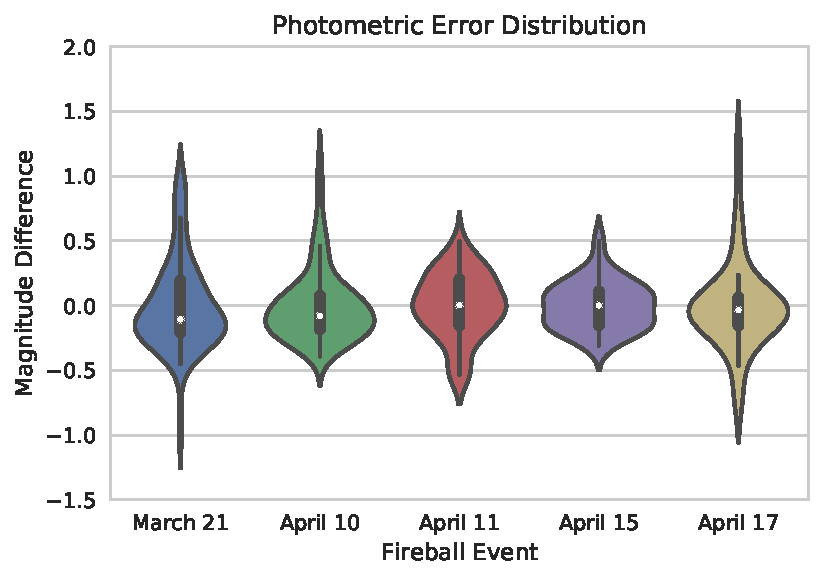
\includegraphics[width=\linewidth]{AllViolins.pdf}
	\label{fig:AllViolins}
\end{subfigure}%
\begin{subfigure}{.5\textwidth}
	\centering
	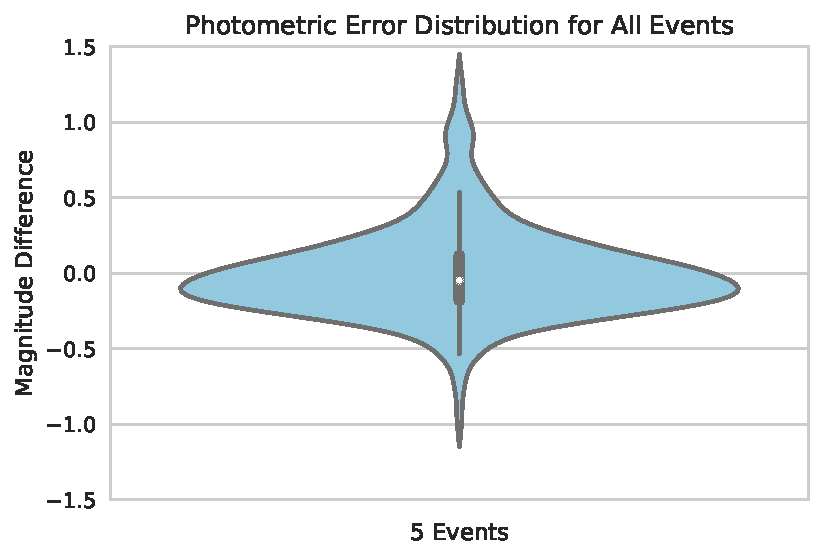
\includegraphics[width=\linewidth]{CombinedViolin.pdf}
	\label{fig:CombinedViolin}
\end{subfigure}
\caption{The violin plot for all these events have a few outliers.}
\label{fig:twoviolin}
\end{figure}


Most of the plots show a few data points do not agree with NASA's light curve. These discrepancy may be because the program does not take into account parameters such as atmospheric extinction. These parameters are more influential if the object moves radially across the night sky in the camera's frame. If NASA did take into account this affect, then that would explain the difference. 

\section{Fireballs detected with D6.}

Ultimately, however, the goal of our research is to show our all-sky camera's capabilities. The final test of the photometry script is thus the ability for it to detect new data collected from our own all-sky camera. With self-collected data, however, there are often problems that requires troubleshooting. One problem that emerged early on in our desire to build an ultra compact and affordable unit was that our hardware was not fast enough to write the frames of the events to the hard drive cleanly. The result of this is incomplete video frames, creating gaps in the data. This can be seen in Figure~\ref{fig:D6Glitch}. 
\begin{figure}[ht!]
	\centering
	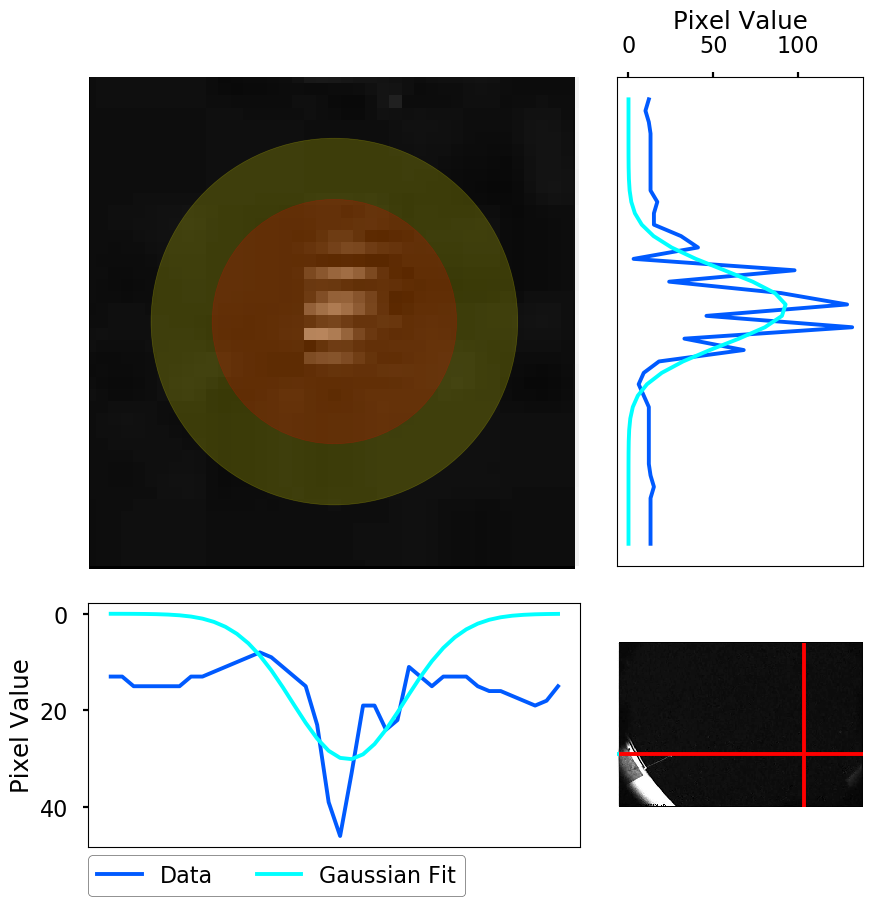
\includegraphics[width=0.4\linewidth]{D6GlitchInverse.png}
	\caption{The incomplete frame data can be seen in both slices of the pixel data.}
	\label{fig:D6Glitch}
\end{figure}
This results in frames with much lower pixel values inside the object's radius than what one would expect, and what it would be if accurately representing the meteoritic phenomenon correctly. This is further seen in the resulting light curve, show in Figure~\ref{fig:D6LightCurve}.

\begin{figure}[ht!]
	\centering
	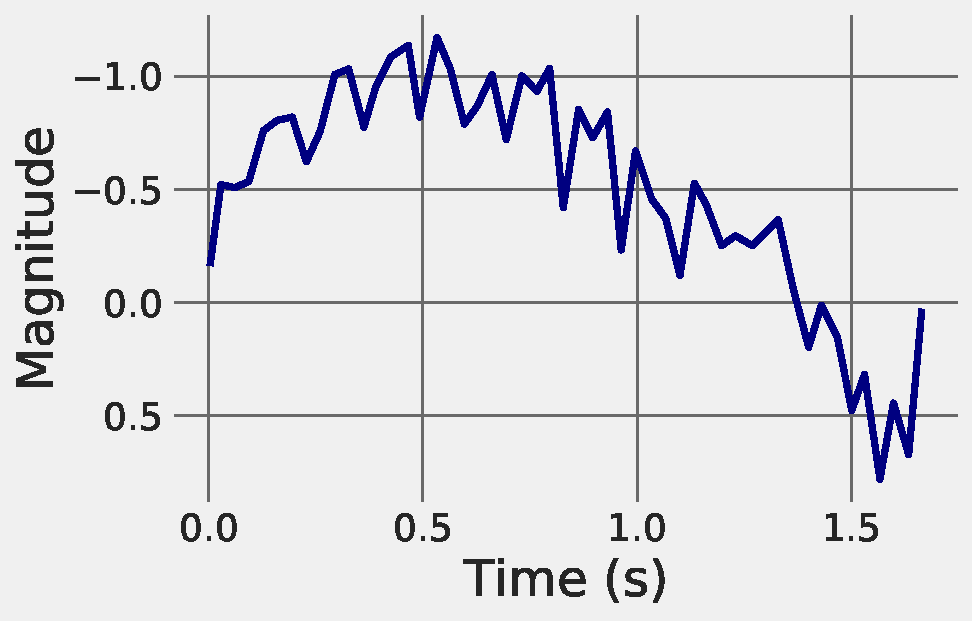
\includegraphics[width=0.6\linewidth]{/home/luke/Data/D6/D6Curve.pdf}
	\caption{The light curve of this event is much less smooth than one would expect from a fireball}
	\label{fig:D6LightCurve}
\end{figure}

It is worth noting that is another possible example of what happens often when we are analyzing a dim event: there is a very high noise to signal ratio. For this reason, along with the previously mentioned ones, this fireball event is not a strong test sample. The program will have to wait until D6's operating system is finished updating before getting another attempt at in-house data. 
